%=== CHAPTER ONE (1) ===
%=== INTRODUCTION ===

\chapter{Introduction}
\begin{spacing}{1.5}
\setlength{\parskip}{0.3in}

In this chapter, I will give the background of the problem that will focus on. In \autoref{sec:IN_background}, I will describe the situation of smart car driving and ADAS system utilization, and state the importance of lane and road marking detection in ADAS system. In \autoref{sec:IN_motivation}, I will explain why I want to solve such a problem and on which specific issues I will be focusing. In \autoref{sec:IN_objectives} I will give the objectives and the scope of my research. In \autoref{sec:IN_contribution} I will briefly introduce the contributions I have done in this work. In \autoref{sec:IN_organisation} I will give the outline of the following chapters.

\section{Background}
\label{sec:IN_background}

In this section, I will explain the background of my purposed problems. I will describe how the smart cars assistant the human drivers by using the Advanced-driver-assistance system (ADAS) system, and how object-detection methods helps ADAS system to perform better.

The era of the smart cars is coming, and Advanced-driver-assistance system plays an important role in it. Object detection technologies are used to improve the performance of Advanced-driver-assistance system.

Smart cars equipped with Advanced-driver-assistance system are popular now. With the development of smart driving and Eco-energy technology, more and more companies began to produce and sale the newly designed, electric-driven, smart-driving assistant cars. Leading companies like TESLA, NIO and QuantumScape made hundreds of thousands of cars every year (till 2020)~\cite{petranek2015we}. With these cars bought by more and more families, the smart cars are no longer a concept for common people, but becomes a daily necessities for everyone, as an alternative to a traditional car. Compared with traditional mechanical fuel vehicle, new smart vehicles have many advantages. They are 'new', not only because they are driven by electric energy, but also because they are equipped with intelligent driving assistance systems, which is usually called Advanced-driver-assistance system (ADAS).

\begin{figure}[ht]
\centering
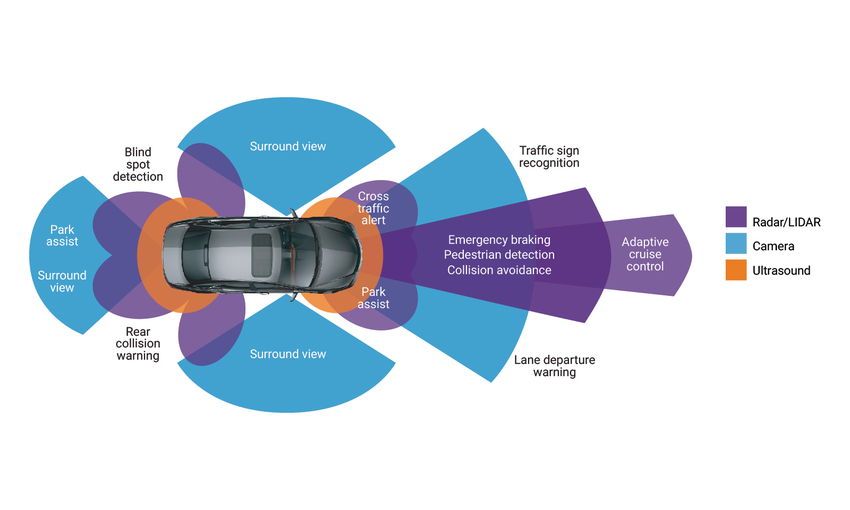
\includegraphics[width=5.5in, fbox]{Chapter1/adas.jpg}
\caption{Advanced Driver Assistance System (ADAS)~\cite{adas}}
\label{fig:adas} 
\end{figure}

ADAS system can reduce road fatalities by minimizing human error. Basic architecture of ADAS system can be shown in \autoref{fig:adas}. Firstly, it utilizes the sensors (LIDAR, in-vehicle camera, GPS) to collect the surrounding obstacle or global position information. Secondly, by combining the information grabbed from all the sensors, the ADAS system can get information that is useful for driving, such as driver's state, current geographical position of cars, the road congestion, potential obstacles on the road, and the trending of road~\cite{morignot2014arbitration}. Such information can be further utilized by the driver or the analysis system to avoid potential dangerous. Because the safety problem is one of the most severe unsolved problems of the traditional human controlled vehicles, ADAS can significantly reduce the death rate related to fatal driving~\cite{brookhuis2001behavioural}.

To improve the performance of ADAS system is an object detection task. ADAS systems use in-vehicle cameras to capture the real-time images of roads~\cite{ziebinski2016survey}. Captured images will be handled by detection module, which recognizes lane outlines and road markings, and then respond to drivers accordingly. This is basically a object detection problem in computer vision area. 

This dissertation work wants to solve the problems raised in the aforementioned background, and the lane-detection method described in this report can be used to improve the performance of ADAS system. 

\section{Motivation}
\label{sec:IN_motivation}

In this section, I will explain why I want to do such a research by describing the specific problems that I want to solve. Example images in this section are selected from VPG database~\cite{lee2017vpgnet}.

There are several common lane detection issues in aforementioned detection process. Two important ones are bad surrounding conditions and the curved road.

First is extreme weather and bad illumination conditions. In raining days, images captured by ADAS’s camera may be blurry or be stained by raindrops as in \autoref{fig:blurry}, and the water on the road may lead to reflection of lights, as shown in \autoref{fig:reflection}. In dusk, sun is dim, and the scene is dark-some. The road markings and lane outlines cannot be distinguished from background easily, as shown in~\autoref{fig:dusk} (in the dusk) and \autoref{fig:night} (in the night) . With such distortions, the detection algorithm cannot see roads accurately. Consequently, taking measures to denoising is of vital importance. 


\begin{figure}[th]
    \centering
    % \begin{adjustbox}{minipage=0.98\linewidth,fbox}
    \begin{subfigure}[b]{0.49\textwidth}
        \centering
        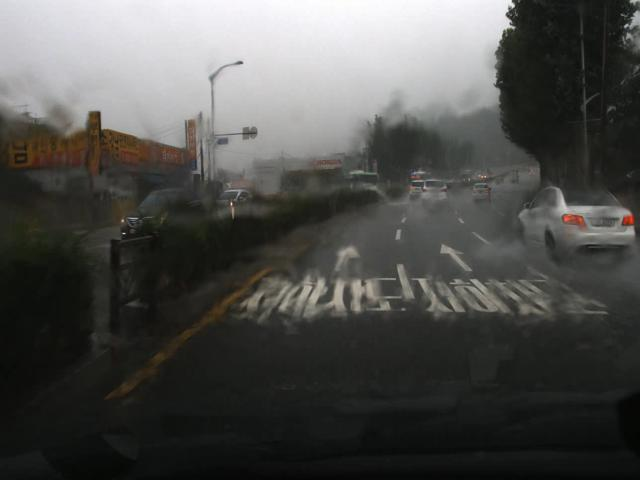
\includegraphics[width=2.7in, fbox]{Chapter1/blurry.png}
        \caption{Blurry Sample}
        \label{fig:blurry} 
    \end{subfigure}%
    ~
    \begin{subfigure}[b]{0.49\textwidth}
        \centering
        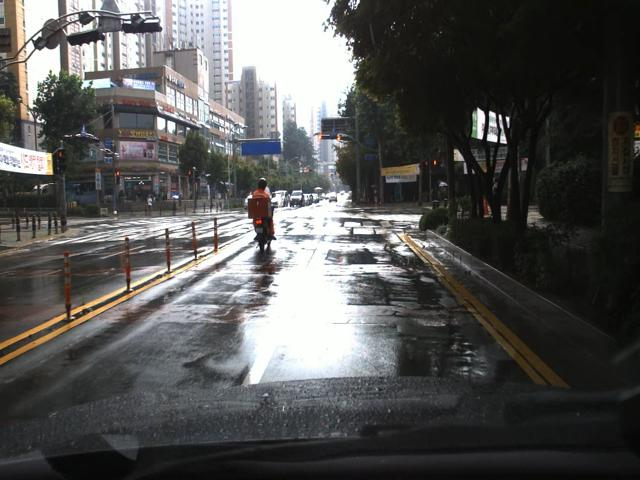
\includegraphics[width=2.7in, fbox]{Chapter1/reflection.png}
        \caption{Reflection Sample}
        \label{fig:reflection} 
    \end{subfigure}
    \\
    \begin{subfigure}[b]{0.49\textwidth}
        \centering
        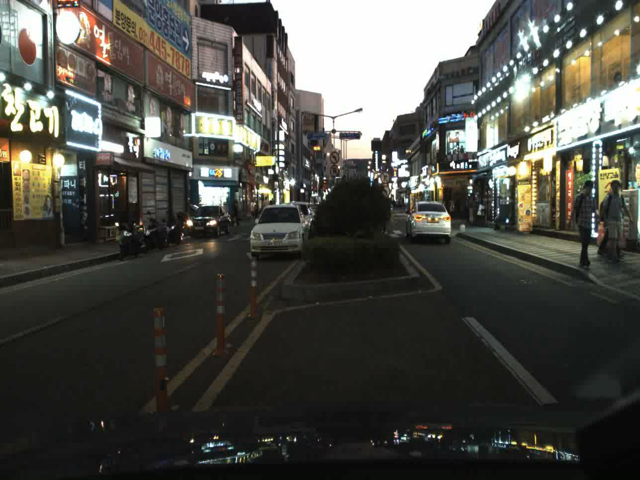
\includegraphics[width=2.7in, fbox]{Chapter1/dusk.png}
        \caption{In the Dusk}
        \label{fig:dusk} 
    \end{subfigure}%
    ~
    \begin{subfigure}[b]{0.49\textwidth}
        \centering
        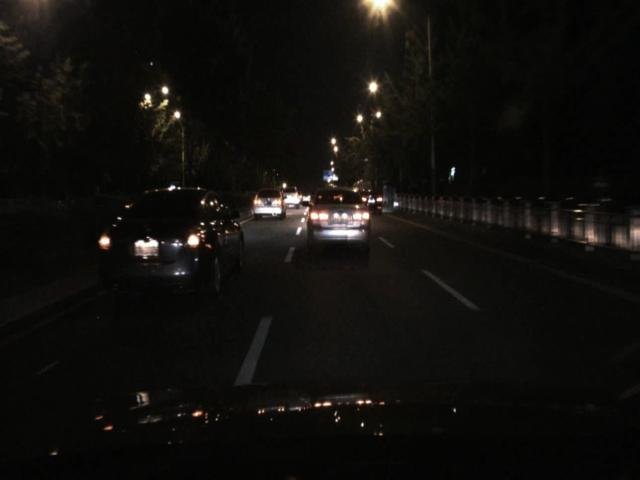
\includegraphics[width=2.7in, fbox]{Chapter1/night.png}
        \caption{In the Night}
        \label{fig:night} 
    \end{subfigure}
    % \end{adjustbox}
    \caption{Extreme Weather and Bad Illumination Condition}
\end{figure}

Second is curved road. Traditional lane detection algorithms usually work well on straight lane but will meet performance drop once the road turns quickly. The comparison of straight road and curved road can be seen in \autoref{fig:straight} and \autoref{fig:curved}.

\begin{figure}[th]
    \centering
    \begin{subfigure}[b]{0.49\textwidth}
        \centering
        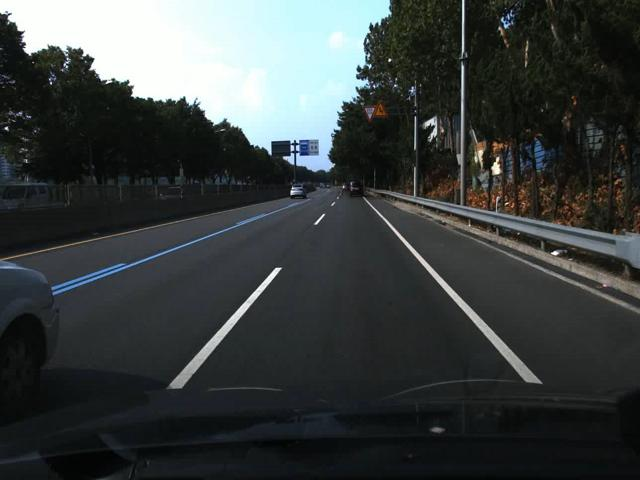
\includegraphics[width=2.7in, fbox]{Chapter1/straight.png}
        \caption{Straight Lane}
        \label{fig:straight} 
    \end{subfigure}%
    ~
    \begin{subfigure}[b]{0.49\textwidth}
        \centering
        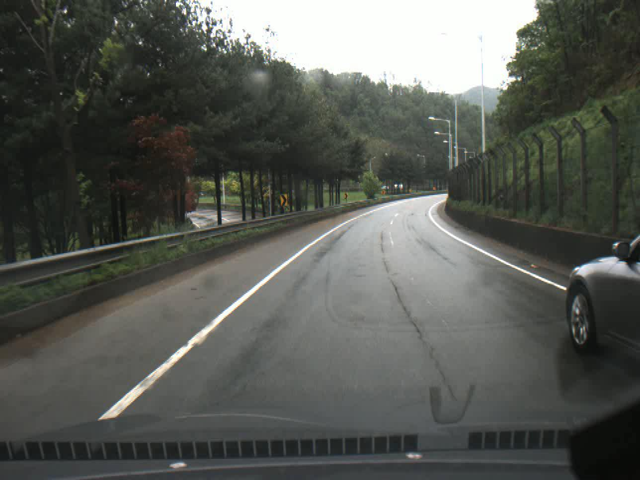
\includegraphics[width=2.7in, fbox]{Chapter1/curved.png}
        \caption{Curved Lane}
        \label{fig:curved} 
    \end{subfigure}
    \caption{Straight and Curved Lane}
\end{figure}

VPGNet~\cite{lee2017vpgnet} used vanishing point information to solve this problem. Vanishing point is the visual intersection of two parallel lines~\cite{barnard1983interpreting}, here it is treated as the unseen end of the road.  Inspired by the intuition that human eyes utilize the vanishing point to predict the road trending, VPGNet tried to feed this information into neural network by multi-task method. They use multi-task because features employed by VP task, like road curving angle and trending, may also be useful in the detection of lanes and road markings. Based on this, we can expect that with VP information given, the Neural Network can converge better on the other two tasks (lane detection, road marking detection). But VPGNet’s VP feeding scheme is simple, not as efficient as expected. In this work, I proposed a new scheme to train with VP information.

The motivation of this research work is to solve above mentioned problems. By solving those problems, ADAS system can perform better in lane detection and road marking recognizing, thus make auto-driving safer.

\section{Objectives and Specifications}
\label{sec:IN_objectives}

In this section, I will claim the aim of my dissertation project and its specifications.

This project aims at developing a Neural Network architecture that can detect the lanes and the road markings on the images, which can be captured by in-vehicle cameras. The input would be 3-channel RGB image, and the output would be a pixel-level classification of the objects in the target image. Totally there are 17 classes of objects, as being listed in \autoref{tab:classes}. Besides, it will predict the vanishing point, which will also guide the prediction of the curving lane. The architecture was implemented both in CAFFE and PyTorch.

\begin{table}[ht]
\centering
\caption{Classes Specification and its Index}
\label{tab:classes}
\begin{tabular}{clcl}
\hline
Index & Lane Type          & Index & Road Marking Type   \\ \hline
0     & Background         & 9     & Stop Line           \\
1     & Lane Solid White   & 10    & Arrow Left          \\
2     & Lane Broken White  & 11    & Arrow Right         \\
3     & Lane Double White  & 12    & Arrow Go Straight   \\
4     & Lane Solid Yellow  & 13    & Arrow U Turn        \\
5     & Lane Broken Yellow & 14    & Speed Bump          \\
6     & Lane Double Yellow & 15    & Cross Walk          \\
7     & Lane Broken Blue   & 16    & Safety Zone         \\
8     & Lane Slow          & 17    & Other Road Markings \\ \hline
\end{tabular}
\end{table}%

The training data mainly comes from two sources. The first is the VPG data set~\cite{lee2017vpgnet}, and the second is the Caltech data set~\cite{aly2008real}.

\section{Major contribution of the Dissertation}
\label{sec:IN_contribution}

This dissertation researched about a pixel-level lane detection and road marking classification Neural Network architecture, which is based on the Fully Convolution Network and multi-task training method. It employs the vanishing points to improve the performance of the lane detection and road marking classification accuracy.

In the data pre-processing, I proposed a data format transition algorithm between two lane data set (VPG data set \cite{lee2017vpgnet} and Caltech data set \cite{aly2008real}), thus the two data set can be translated into same data format, by which format can be fed into either the CAFFE or the PyTorch framework. In the data post-processing, I proposed a multi-class visualization algorithm which gives each class distinguishable color and annotate each pixel with its corresponding color.

In the network architecture part, two brand new combination layers are described. One is the tilling layer which works as an alternative to the traditional concatenate layer with more efficiency. Another one is the 4-map combination layer which feeds the Vanishing Points to the model. The network is implemented in both CAFFE and PyTorch. 2-D Gaussian function are also used to enhance the prediction of the vanishing points.

After the training process, I discussed the threshold of confidential and data point extension method, which will affect the efficiency of the model when applied in practice.

\section{Organisation of the Dissertation}
\label{sec:IN_organisation}

The following chapters will be organized as below.

{\large\textbf{Chapter 2: Literature Review}}

In the \autoref{cha:literature}, I review some of the background theories and algorithms related to object detection in lane and road marking recognition. In \autoref{sec:LR_overview}, I give an over view of history of deep learning networks used in object detection. In \autoref{sec:LR_FCN}, I described the basic theory of Fully Convolution Network and its working mechanism. In \autoref{sec:LR_objectdetection} I discussed the history of object detection algorithms and introduced some of famous ones. In \autoref{sec:LR_vpinNN} I introduced the concept of Vanishing Point and its usage in other lane detection tasks.

{\large\textbf{Chapter 3: Vanishing Point Directed Lane Detection}}

In the \autoref{cha:model}, I introduced the network architecture of my proposed Neural Network, and also the detailed specifications in training. In \autoref{sec:MD_model}, I introduced the main network structure and its multi-task configuration. In \autoref{sec:MD_CAFFE}, I introduced the training process of the CAFFE implementation, its environment configuration and some user-defined layers used. In \autoref{sec:MD_PyTorch}, I introduced the PyTorch implementation of this network and data transition procedure.

{\large\textbf{Chapter 4: Improvements}}

In the \autoref{cha:improvements}, I introduced some improvements done based on the base network. In \autoref{sec:IM_2D} I introduced a new scheme which uses 2-D Gaussian function to make the single point data being fed into the model efficiently and why I have to do so. In \autoref{sec:IM_resblock} I  introduced how to imply residual blocks to increase the FCN network learning accuracy. In \autoref{sec:IM_Enet} I introduced the E-Net and the part that being used in our model.

{\large\textbf{Chapter 5: Experimental Results and Discussion}}

In the \autoref{cha:experiments}, I discussed the experiment results of the model. I gave the mathematical equations of the test metrics. After that, I introduced a visualization tool that can be used to annotate the pixel-level classification images. Then, I analyzed the experimental outputs in normal condition and in rainy condition. Finally, I discussed the confidential threshold selection of the prediction result.

{\large\textbf{Chapter 6: Conclusion and Recommendations}}

In the \autoref{cha:conclusion}, I summarized my work and gave the conclusion. I also gave some future work recommendation in the last section.

\end{spacing}
%=== END OF CHAPTER ONE ===
\newpage


